\section{Proposed NeST-Com Framework}
\subsection{Next-Scale Representation and Digital Frame}
We transmit $x\in[0,1]^{256\times256\times3}$ over complex AWGN,
\begin{equation}
 y=s+n,\quad n\sim\mathcal{CN}(0,\sigma^2 I_N),\quad
 \mathrm{SNR}=10\log_{10}(E_s/\sigma^2),
 \label{eq:channel}
\end{equation}
using $N$ complex symbols per image and nominal $E_s=2$. TX selects a frozen policy for the channel SNR; RX uses the true noise variance for LLRs. Digital constellations have average energy two without per-frame renormalization. Continuous JSCC data are normalized per image to average energy two, with required Swin side information paid within $N$. A 12-bit profile ID, CRC16, and terminated rate-1/2 convolutional code occupy 68 rotated-BPSK symbols $\{\pm(1+j)\}$. The remaining $N-68$ symbols carry the LDPC-coded body. The paid profile identifies the actual endpoint and MCS. Our main budget is $N=1024$; the reduced-budget experiment uses $N=512$ without increasing $E_s$.

The frozen VAR tokenizer produces ten residual token maps $q_s$, with side lengths $(1,2,3,4,5,6,8,10,13,16)$ and a 4096-entry codebook~\cite{var}. Let $L_s$ be the map size and $C_s$ its codebook lookup, resizing, and residual transform. Complete coarse maps span the whole latent grid after resizing; the sum $f_q=\sum_s C_s(q_s)$ accumulates their residual refinements. Image decoder $\Dc$ is adapted on 20\,000 ImageNet training images using continuous, fully quantized, and prefix-completion-interpolated latents, then fixed. NeST-Com uses null-class conditioning. Its frozen next-scale prior factorizes as
\begin{equation}
 p_\theta(q_s\mid q_{<s})=\prod_{i=1}^{L_s}p_\theta(q_{s,i}\mid q_{<s}),
 \label{eq:prior}
\end{equation}
providing local cumulative distribution functions (CDFs) for arithmetic coding~\cite{arithmetic} at both ends of Fig.~\ref{fig:system}.

\begin{figure*}[t]
\centering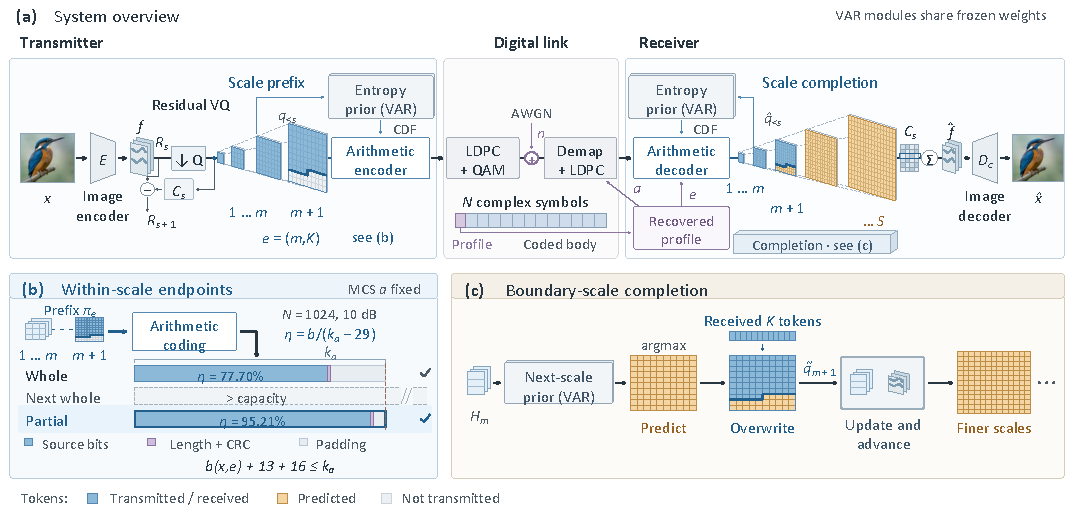
\includegraphics[width=\textwidth]{figure1.pdf}
\caption{NeST-Com. (a) The paid profile specifies endpoint $e$ and MCS $a$; TX/RX construct CDFs from the shared frozen VAR and their known coarse tokens. (b) Independently terminated prefixes, a 13-bit length field, and CRC16 fit $k_a$. Bars show common500 entropy-stream capacity utilization at $N=1024$, 10~dB (WHOLE 77.70\%; PARTIAL 95.21\%). (c) Received positions overwrite the predicted boundary map before residual accumulation and advancement to finer scales. $H_m$ denotes the prior state after scale $m$.}
\label{fig:system}
\end{figure*}

\subsection{Within-Scale Endpoints and Actual-Length Fitting}
An endpoint $e=(m,K)$ retains complete coarse maps and $K$ raster-ordered positions from the next map:
\begin{equation}
 \pi_e=(q_1,\ldots,q_m,q_{m+1,1:K}).
 \label{eq:prefix}
\end{equation}
WHOLE permits $K=0$ for $m=4,\ldots,10$. PARTIAL adds
$K\in\{\lfloor L_{m+1}/4\rfloor,\allowbreak\lfloor L_{m+1}/2\rfloor,\allowbreak\lfloor3L_{m+1}/4\rfloor\}$ for $m=4,\ldots,9$, giving 25 endpoints in total. $(10,0)$ is the full representation.

For MCS $a=(M,r)$, the coded body has $n_a=(N-68)\log_2M$ bits and information length $k_a=\lfloor rn_a\rfloor$. With actual terminated arithmetic length $b(x,e)$,
\begin{equation}
 b(x,e)+29\leq k_a,\qquad \eta(x,e)=\frac{b(x,e)}{k_a-29}.
 \label{eq:budget}
\end{equation}
The 29 bits comprise the length field and CRC16; unused information positions are zero-padded before 5G NR LDPC coding, rate matching~\cite{nr}, and QAM. Thus $\eta$ measures entropy-stream capacity utilization.

Offline calibration selects a target endpoint and MCS for each budget/SNR. A 100-image pilot uses one channel realization per image; the finalists are evaluated on all 1000 calibration images with three realizations per image. Selection maximizes source/reconstruction DINOv2 cosine~\cite{dinov2}, averaged over realizations first and then equally over sources, including gray failures. Exact ties use a fixed candidate order. At $N=1024$, target screening starts at scales 7--9 and includes full-scale $(10,0)$ candidates in final evaluation. At $N=512$, WHOLE/PARTIAL screen all 7/25 targets against the same 12 MCSs, $\log_2M\in\{2,4,6\}$ and $r\in\{1/2,2/3,3/4,5/6\}$. Each method/SNR advances the top three plus a maximum-endpoint QPSK rate-1/2 anchor. Ada uses the same N512 MCS pool with longest-feasible fitting up to 256 tokens. The full candidate and selection rules are provided with the results.

Online fitting fixes the selected MCS and searches legal endpoints no longer than the target, in decreasing token count down to $(4,0)$. TX sends the first independently terminated stream satisfying~\eqref{eq:budget}; the paid profile identifies the actual endpoint. Arithmetic streams are never cut from longer streams. If no endpoint fits, the N512 protocol sends a paid NULL profile and short NULL payload through the complete frame, retaining a gray reconstruction in the denominator. The N1024 implementation instead raises an error; no evaluated N1024 source encountered this case.

\subsection{Prefix-Constrained Reconstruction}
Invalid profile CRC/catalogue, body CRC, declared length, known padding, or arithmetic parsing produces a fixed gray image; so does a valid N512 NULL reception. Otherwise, RX decodes the prefix using CDFs rebuilt from received complete coarse maps. It predicts the boundary map by VAR argmax conditioned on those maps, then applies known-token overwrite~\cite{var}:
\begin{equation}
 \tilde q_{m+1,i}=\begin{cases}\hat q_{m+1,i},&i\leq K,\\q^{\mathrm{pred}}_{m+1,i},&i>K.\end{cases}
 \label{eq:overwrite}
\end{equation}
Unreceived boundary positions retain their coarse-conditioned prediction. The merged map contributes to the residual latent and updates the prior state before finer-scale prediction. Complete received maps remain unchanged; subsequent maps are generated from this updated context. Reconstruction is
\begin{equation}
 \hat x=\Dc\!\left(\sum_{s=1}^{10}C_s(\tilde q_s)\right).
 \label{eq:reconstruction}
\end{equation}
At the final scale, overwrite changes the residual contribution without any subsequent propagation.
